\documentclass{article}%
\usepackage[T1]{fontenc}%
\usepackage[utf8]{inputenc}%
\usepackage{lmodern}%
\usepackage{textcomp}%
\usepackage{lastpage}%
\usepackage{authblk}%
\usepackage{graphicx}%
%
\title{A novel function for p21Cip1 and acetyltransferase p/CAF as critical transcriptional regulators of TGFb{-}mediated breast cancer cell migration and invasion}%
\author{Kylie Perez}%
\affil{Department of Neurology, The Agnes Ginges Center for Human Neurogenetics, Hadassah University Hospital, Jerusalem, Israel}%
\date{01{-}01{-}2012}%
%
\begin{document}%
\normalsize%
\maketitle%
\section{Abstract}%
\label{sec:Abstract}%
A novel therapy inspired by the innate immune system of breast cancer cells to activate protein kinase (miK) recognizes a mutant cellular protein, LKB1, and disrupts it in a targeted inflammatory state. This anti{-}cancer protein kinase gene{-}messenger is activated through a LKB1{-}dependent pathway when both of the molecules, LKB1 and miK1, interact with each other.\newline%
This therapeutic is pre{-}clinical in human breast cancer cells via a LKB1{-}driven pathway, with promising results. In addition, miK1{-}dependent miK activity was protected when expressing the LKB1{-}literal lineage of miK1. Moreover, this specific type of LKB1 is expressed in patients with HER2 cancer associated with primary tumor cells and spontaneously proliferates in lymph nodes where the cells are genetically programmed to divide, as reported in the journal Molecular Immunology.\newline%
"Our study is the first to demonstrate that tumors with lkb1{-}deficient cells can have mutations in the miK1{-}regulated pathway, allowing for proliferation and ultimately growth," said Wei{-}Chang Chiu, Ph.D., a research assistant professor in the Department of Pathology, first author of the study and associate professor of microbiology and immunology at UCSF. "This means that miK1{-}based therapies that selectively interact with miK1{-}deficient cell types may be an effective strategy in treating breast cancer."\newline%
Chiu added, "Our work suggests that, in this mode of microenvironment modification, these tumors with lkb1{-}deficient breast cancers might be able to evolve into other diseases, such as liver cancer and non{-}Hodgkin lymphoma, by directly targeting the genetically programmed cells."\newline%
In addition to using LKB1{-}driven miK1{-}mediated metabolic activation in mouse breast cancer cells, Chiu also distinguished engineered cancer cells to display completely identical metabolite signaling patterns as monoclonal antibodies manufactured by the NIH Avastin/CSF Consortium for HER2{-}expressing breast cancer cells. The researchers believe that other molecular fingerprint discovery and targeting teams may be developing similar molecules using the LKB1/LKB1 pathway in breast cancer tumors, using similar mechanisms of molecular regulation and targeting.\newline%
"We are discovering more and more properties of the LKB1 pathway, based on the synergy between miK1 and miK1. In many instances, mutations in LKB1{-}deficient cell types were critical to tumor growth," said Hans Vogelsang, Ph.D., co{-}author of the study and professor in the Department of Pathology, first author of the study and associate professor of microbiology and immunology at UCSF. "We are still exploring more therapeutic strategies for specific chemotherapy regimens, such as those that target tumor{-}destructing genes, such as HER2{-}deficient cells."

%
\subsection{Image Analysis}%
\label{subsec:ImageAnalysis}%


\begin{figure}[h!]%
\centering%
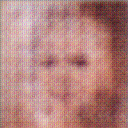
\includegraphics[width=150px]{500_fake_images/samples_5_407.png}%
\caption{A Close Up Of A Black And White Cat}%
\end{figure}

%
\end{document}